\documentclass[11pt, a4paper, titlepage]{article}

% packages

\usepackage[utf8]{inputenc}
\usepackage[T1]{fontenc}

\usepackage{amsmath}
\usepackage{amsfonts}
\usepackage{amssymb}
\usepackage{setspace}
\usepackage{wrapfig}
\usepackage{cite}
\usepackage{indentfirst}
\usepackage{subcaption}

%% packages and package-dependent commands

\usepackage{graphicx}
\graphicspath{{./images/}}

\usepackage[thmmarks]{ntheorem}

\theorembodyfont{\normalfont}
\theoremseparator{.}
\theoremindent0.5cm
\theoremnumbering{arabic}
\theoremsymbol{\ensuremath{\ast}}
\newtheorem{definition}{Definition}

\usepackage{xargs}

\usepackage[pdftex, dvipsnames, hyperref]{xcolor}

\definecolor{mnk_blue}{rgb}{.2, .56, 1}
\definecolor{mnk_red}{rgb}{.9, .16, .1}
\definecolor{mnk_orange}{rgb}{.99, .59, .12}
\definecolor{mnk_yellow}{rgb}{.9, .86, .45}

\makeatletter
\usepackage[pdfusetitle]{hyperref}
\hypersetup{colorlinks, urlcolor=mnk_blue, citecolor=black, filecolor=black,
            linkcolor=black, linktoc=page,
            pdfsubject={Algorithms on graphs; Persistent Phylogeny}}
\makeatother

\usepackage[
  colorinlistoftodos,
  prependcaption,
  backgroundcolor=mnk_yellow,
  linecolor=mnk_yellow,
  textsize=tiny
]{todonotes}

\newcommandx{\fix}[2][1=]{%
  \todo[backgroundcolor=mnk_red, linecolor=mnk_red, #1]{#2}
}

\newcommandx{\wip}[2][1=]{%
  \todo[backgroundcolor=mnk_orange, linecolor=mnk_orange, #1]{#2}
}

\usepackage{tikz}

\usepackage{relsize}

\newcommand*{\cc}{%
  C\nolinebreak[4]\hspace{-.05em}%
  \raisebox{.4ex}{\relsize{-3}{\textbf{++}}}%
}

\newcommandx*{\m}[2][1, 2]{\ensuremath{{M_{#1}}_{#2}}}
\newcommand*{\ma}{\ensuremath{(M, A)}}

\newcommandx*{\species}[2][1, 2]{\ensuremath{s_{#1}^{#2}}}
\newcommandx*{\character}[2][1, 2]{\ensuremath{c_{#1}^{#2}}}

\newcommand*{\g}{\ensuremath{G}}
\newcommand*{\grb}{\ensuremath{G_{RB}}}
\newcommand*{\edge}[2]{\ensuremath{(#1, #2)}}

% information

\author{Davide Casella}
\title{Efficient algorithms to compute a Persistent Phylogeny}

% body

\begin{document}
  \hypersetup{pageanchor=false}

  %!TEX root = ../thesis.tex

\makeatletter

\begin{titlepage}

  \begin{spacing}{1.48}
    \begin{wrapfigure}[5]{l}[20mm]{0.2\linewidth}
      
\includegraphics[width=\linewidth]{bicocca.png}
    \end{wrapfigure}
    \text{} \\[-0.027\textheight]
    Università degli Studi di Milano Bicocca \\
    \textbf{Scuola di Scienze} \\
    \textbf{Dipartimento di Informatica, Sistemistica e Comunicazione} \\
    \textbf{Corso di laurea in Informatica}
  \end{spacing}

  \vfill

  \begin{spacing}{2}
    \begin{center}
      {\huge \textbf{\@title}}
    \end{center}
  \end{spacing}

  \vfill

  \begin{onehalfspace}
    \begin{flushleft}
      {\large \textbf{Relatore:}    \textit{Prof. Paola Bonizzoni} \\
              \textbf{Co-relatore:} \textit{Prof. Gianluca Della Vedova}}
    \end{flushleft}
  \end{onehalfspace}

  \vfill

  \begin{onehalfspace}
    \begin{flushright}
      {\large \textbf{Relazione della prova finale di:} \\
              \textit{\@author} \\
              \textit{Matricola 793631}}
    \end{flushright}
  \end{onehalfspace}

  \vfill

  \begin{center}
    {\large \textbf{Anno Accademico 2016--2017}}
  \end{center}

\end{titlepage}

\makeatother


  %!TEX root = ../thesis.tex

\begin{abstract}

  Recently, studying character-based phylogeny models that allow the loss of characters gained relevancy.
  E.g., in tumor phylogeny, the deletion of entire genomic regions often cause loss of (previously acquired) mutations.

  The Persistent Phylogeny model solves this by generalizing the concept of Perfect Phylogeny, allowing for each character to be acquired and lost at most once during the evolutionary events.

  We formalize and contextualize this problem, describing a recently introduced algorithm for reconstructing a Persistent Phylogeny tree starting from a binary matrix, the first solving this problem in polynomial time.

  We then proceed to implement it using the \cc{} language and Boost libraries, complementing the study with tests on instances that do or don't admit a Persistent Phylogeny, and performance evalutation.

\end{abstract}


  \tableofcontents
  \thispagestyle{empty}

  \pagebreak

  \listoftodos          % temporary - delete
  \thispagestyle{empty} % temporary - delete
  \pagebreak            % temporary - delete

  \hypersetup{pageanchor=true}
  \setcounter{page}{1}

  %!TEX root = ../thesis.tex

\section{Introduction}\label{sec:introduction}

Reconstructing character-based phylogenies, which are used to study the evolution of characters shared by a collection of species (taxa or individuals), is a recurring problem in Bioinformatics, mainly due to the complexity of the task. In fact, there exist multiple approaches to evolutionary history reconstruction; most of those approaches try to reduce the problem by limiting the way (or amount of times) characters can change state in the phylogenetic tree. The Persistent Phylogeny model, which we will talk about in the following sections, allows characters to be acquired and lost at most once in the evolutionary history.

\subsection{Character evolution in Bioinformatics}\label{ssec:charevo}

To study the state changes of characters in an evolutionary tree we can represent species and their characters as rows and columns of a matrix; each element of the matrix marks the specific state of a character for a species.

We will consider the case in which all characters are binary, making them able to assume only one of two states, 0 or 1. For each species, the state of a character represents if the species has or doesn't have a given feature.

\begin{definition}\label{def:m}
  \m{} is a $n \times m$ binary matrix over a set $m$ of characters and a set $n$ of species.

  \m[i][j] represents the state of a character \character[j] for a species \species[i].
\end{definition}

A matrix \m{} can then be represented as an undirected bipartite graph. The set of vertices of the graph is $S \cup C$, where $S$ is the set of species and $C$ the set of characters.

\begin{figure}[h]
  %!TEX root = ../thesis.tex

\begin{subfigure}[b]{0.45\textwidth}
  \centering
    \begin{tabular}{c | c c c c}
      \m{}  & $c_0$ & $c_1$ & $c_2$ & $c_3$ \\ \hline
      $s_0$ & 0     & 1     & 1     & 1     \\
      $s_1$ & 0     & 0     & 0     & 1     \\
      $s_2$ & 1     & 1     & 0     & 0     \\
      $s_3$ & 1     & 0     & 1     & 0
    \end{tabular}

  \caption{Matrix for the instance}\label{figure:1:a}
\end{subfigure}
\hfill
\begin{subfigure}[b]{0.45\textwidth}
  \centering
    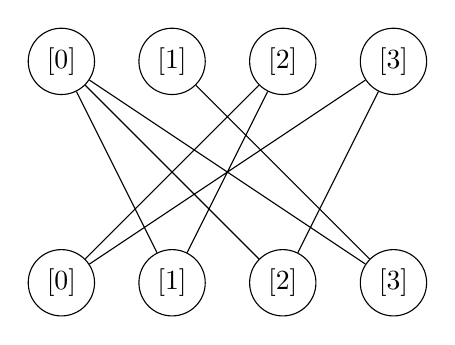
\begin{tikzpicture}
      {\tikzstyle{every node}=[circle, draw]
        \foreach \i in {0, ..., 3}
        {
          \node (s\i) at (\i*40pt, 80pt) {\species[\i]};
        }

        \foreach \j in {0, ..., 3}
        {
          \node (c\j) at (\j*40pt, 0) {\character[\j]};
        }
      }

      \draw
        (c0) -- (s2)
        (c0) -- (s3)
        (c1) -- (s0)
        (c1) -- (s2)
        (c2) -- (s0)
        (c2) -- (s3)
        (c3) -- (s0)
        (c3) -- (s1);
    \end{tikzpicture}

  \caption{Graph for the instance}\label{figure:1:b}
\end{subfigure}


  \caption{An instance of a character-based phylogeny represented as matrix and graph $(\text{4 species} \times \text{4 characters})$}
  \label{fig:1}
\end{figure}

In the figure above (\ref{fig:1}) we have a set of species $S = \{ \species[0], \species[1], \species[2], \species[3] \}$ and a set of characters $C = \{ \character[0], \character[1], \character[2], \character[3] \}$.
Each element $\m[i][j] = 1$ of the matrix (\ref{fig:1:a}) is shown as the edge \edge{\species[i]}{\character[j]} in the corresponding graph (\ref{fig:1:b}).

\subsubsection{Character states}\label{sssec:charstates}

\todo[inline]{Characters can be gained or lost}

Let us introduce the concept of \textit{active} characters.
Active characters \wip{Go on} \dots

\subsection{Persistent Phylogeny problem}\label{ssec:ppp}

\wip[inline]{Add biology PP description \\
             Add PP matrix description}

Each instance of a PPP is associated to a pair \ma{}.

\fix{Sentence start} \dots formalizing input and output parameters for the Persistent Phylogeny problem (PPP) \cite{Bonizzoni2016SolvingTP}.

\begin{definition}[Persistent Phylogeny problem]\label{def:ppp}
  \text{}

  \textit{Input:} pair \ma{} where \m{} is a $n \times m$ binary matrix over a set $m$ of characters and a set $n$ of species, and A is a subset of its characters.

  \textit{Output:} tree $T$ solving \m{} if it exists.
\end{definition}

\subsubsection{Red-black graph representation}\label{sssec:grb}

A red-black graph for an instance of PPP is an undirected bipartite graph whose edges are colored as either red or black.

\begin{definition}[Red-black graph for PPP]\label{def:grb}
  Let $S$ be a set of species vertices, $C$ a set of character vertices, $E$ a set of edges, $A$ a subset of character vertices (active characters).
  Then \grb{} is defined as follows:

  \[ \grb{} = (S, C, E, A) \]

  The vertex set of \grb{} is formally represented as two disjoint and independent sets $S$ and $C$.
\end{definition}

\todo[inline]{GRB and T are in relation thanks to the c-reduction}

A \textit{c-reduction} for a graph \grb{} is the sequence of operations that, when performed on an instance of PPP, clears the graph of all edges.


  \pagebreak % temporary - delete

  %!TEX root = ../thesis.tex

\section{Algorithm explaination}\label{section:algorithm}

The polynomial-time algorithm introduced in \cite{PPPptime2016} describes a recursive procedure for reducing a red-black graph to an empty graph, if it admits a persistent phylogeny.
The recursion stops either when the base case is reached - empty graph (line \ref{algorithm:reduce:ifempty}) - or when the algorithm can't compute a successful c-reduction for \grb{} - the graph reaches a state of irreducibility (line \ref{algorithm:reduce:ifnosource}).

The procedure for a Reduce function is given below.

\begin{algorithm}[h]
  \caption{Reduce. Recursive reduction of a red-black graph.}\label{algorithm:reduce}

  \SetKwData{Source}{\ensuremath{s}}
  \SetKwData{Sc}{\ensuremath{S_{c}}}
  \SetKwInOut{Input}{Input}
  \SetKwInOut{Output}{Output}

  \Input{Red-black graph \grb{}}
  \Output{c-reduction of the graph \grb{}, if it exists}

  \BlankLine

  Remove singletons from \grb{}\;\label{algorithm:reduce:rmsingle}

  \If{\grb{} is empty}{\label{algorithm:reduce:ifempty}
    \Return $\langle$ $\rangle$\;
  }

  \BlankLine

  \If{\grb{} has a free character \character{}}{\label{algorithm:reduce:iffree}
    \grb{} $\gets$ Realize(\character[][-], \grb{})\;

    \Return $\langle$ \character[][-], Reduce(\grb{}) $\rangle$\;
  }

  \BlankLine

  \If{\grb{} has a universal character \character{}}{\label{algorithm:reduce:ifuniversal}
    \grb{} $\gets$ Realize(\character[][+], \grb{})\;

    \Return $\langle$ \character[][+], Reduce(\grb{}) $\rangle$\;
  }

  \BlankLine

  \If{\grb{} has k > 1 connected components}{\label{algorithm:reduce:ifdisconnected}
    \Return $\langle$ Reduce($\grb{}_{0}$), \dots, Reduce($\grb{}_{k-1}$) $\rangle$\;
  }

  \BlankLine

  \gm{} $\gets$ maximal reducible graph of \grb{}\;

  \hasse{} $\gets$ Hasse diagram for \gm{}\;

  \BlankLine

  \If{\hasse{} has no safe source}{\label{algorithm:reduce:ifnosource}
    Abort\;
  }

  \BlankLine

  \Source $\gets$ Find-initial-state(\hasse{})\;

  \Sc $\gets$ sequence of positive characters of \Source that are inactive in \grb{}\;

  \grb{} $\gets$ Realize(\Sc, \grb{})\;

  \BlankLine

  \Return $\langle$ \Sc, Reduce(\grb{}) $\rangle$\;
\end{algorithm}

The Reduce procedure computes signed character realizations with the support of a Realize function, which follows the definition of Realization (\ref{definition:realization}) and extends it to support a list of signed characters as input. We describe the procedure for the Realize function.

\pagebreak % temporary - delete

\begin{algorithm}[h]
  \caption{Realize. Realization of a list of signed characters in a red-black graph.}\label{algorithm:realize}

  \SetKwData{Lc}{\ensuremath{L_{c}}}
  \SetKwData{Con}{\ensuremath{Conn(\character{})}}
  \SetKwData{Adj}{\ensuremath{S(\character{})}}
  \SetKwInOut{Input}{Input}
  \SetKwInOut{Output}{Output}

  \Input{List of signed characters \Lc of \grb{}}
  \Input{Red-black graph \grb{}}
  \Output{Red-black graph \grb{} after the realization of \Lc, if feasible}

  \BlankLine

  \ForEach{\character[][\pm] $\in$ \Lc}{
    \Con $\gets$ species in the connected component that contains \character{}\;
    \Adj $\gets$ species adjacent to \character{}\;

    \BlankLine

    \If{\character[][+] is inactive}{
      Add red edges between \character{} and each species in $\Con \setminus \Adj$\;

      Delete black edges incident on \character{}\;
    }
    \ElseIf{\character[][-] is active}{
      Delete edges incident on \character{}\;
    }
    \Else{
      Abort\;
    }
  }

  \BlankLine

  \Return \grb{}\;
\end{algorithm}

Notice that a realization may alter the connected components of the red-black graph; we then need to recompute (or update) the connected component of a character \character[][\pm] before its realization.

To ensure that a character external to $L_{c}$ gets realized whenever possible, the procedure can be extended by adding checks for free and universal characters after each realization.

Finally, a step that removes singletons from the red-black graph can be implemented right before the \textbf{return} statement.

We will address the Find-initial-state procedure in detail in section \ref{section:safe-chains-sources}.

\subsection{Preparing the graph}\label{section:preparing-the-graph}

An explaination of lines \ref{algorithm:reduce:rmsingle} to \ref{algorithm:reduce:ifdisconnected} has already been provided in section \ref{section:grb}.

The first steps of the Reduce procedure (algorithm \ref{algorithm:reduce}) serve the purpose of bringing the red-black graph to a state which can't be "pruned" further.
Removing isolated vertices (singletons), realizing free and universal characters, and reducing each connected component of \grb{} separately is all part of preparing the graph for a more thorough analysis.

\subsection{Maximal reducible graph and Hasse diagram}\label{section:gm-hassediagram}

Let us introduce the concept of \emph{maximal} character. A character \character{} is maximal in a red-black graph \grb{} if $S(\character{}) \not\subset S(\character[i])$ for each inactive character \character[i] of \grb{}. Two maximal characters \character[0] and \character[1] can overlap, i.e., share common species, but clearly they can't be included in one another. Moreover, to clarify what we just described, we say that a character \character[0] includes another character \character[1] if $S(\character[0]) \supseteq S(\character[1])$.

The set of maximal characters of \grb{} is then used to build a maximal reducible graph \grbcm{} from it.

\begin{definition}[Maximal reducible graph]\label{definition:maximal-reducible-graph}
  Let \grb{} be a red-black graph and \cm{} its set of maximal characters.

  The maximal reducible graph \grbcm{}, \gm{} for short, is the red-black graph induced in \grb{} by the set \cm{} of characters.

  \gm{} consists of the subgraph of \grb{} that has the characters in \cm{} and the species of \grb{} adjacent to \cm{}.
\end{definition}

\todo[inline]{Hasse diagram}

\subsection{Safe chains and sources}\label{section:safe-chains-sources}


  \pagebreak % temporary - delete

  %!TEX root = ../thesis.tex

\section{Algorithm implementation}\label{section:implementation}

\subsection{Language choices}\label{section:language-choices}

\subsubsection{Boost libraries}\label{section:boost-libs}

\paragraph{Boost Graph}

\paragraph{Boost Bimap}

\paragraph{Boost Program Options}

\paragraph{Boost Python}

\subsection{Program options}\label{section:program-options}

\subsection{Boost Graph classes}\label{section:graph-classes}

\subsubsection{RBGraph class}\label{section:rbgraph-class}

\paragraph{Traits and properties}

\paragraph{General purpose functions}

\paragraph{Algorithm functions}

\subsubsection{HDGraph class}\label{section:hdgraph-class}

\paragraph{Traits and properties}

\paragraph{General purpose functions}

\subsection{Algorithm functions}\label{section:algorithm-functions}

\subsubsection{Realize characters and species}\label{section:realize}

\subsubsection{Find initial state(s)}\label{section:initial-state}

\subsubsection{Reduce}\label{section:reduce}


  \todo[inline]{Add section to talk about the performed tests}

  \pagebreak % temporary - delete

  %!TEX root = ../thesis.tex

\section{Conclusions}\label{section:conclusions}

\subsection{Implementation improvements}\label{section:impl-improvements}

\todo[inline]{Find a better way to X}

\subsubsection{Bottlenecks}\label{section:bottlenecks}

\todo[inline]{Repeated connected components}

\subsection{Further development}\label{section:further-dev}

\todo[inline]{Expand to minimal characters}


  \pagebreak

  \bibliographystyle{abbrv}
  \bibliography{bibliography}
\end{document}
